
    \section{Software choices}
        The first part of the workflow is to design a simulation platform. Pre-existing physics engines such as PyBullet or Gazeboo framework are well known in the simulation field. The reason why a new platform was created is that the idea is not to use a physics engine, but rather a mathematical solver for a specific scenario, the multistable joint based robot. Also by building a specific implementation, we can specifically add or remove modules that will analyze simpler or more complex scenarios. It also helps controlling output validity as the hypothesis that has been made during the implementation are known. With those facts, it was decided to build a specific framework.\\
        
        The choice of the programming language is determined by the tasks that need to be achieved, which are characterized by equation solving and ease of modular design. This leaves two main languages, Python and Matlab, both are very similar but Python is well known regarding machine learning tools available and thus Python gives us more flexibility for the controller that involves machine learning. Based on those points, the choice of Python as the main language is obvious.
    
    \section{Program structure}\label{sec:program_structure}
        The framework is built using Python 3. This allows to create modularity in the simulation's structure. Figure \ref{fig:code_structure} describe each physical part of the robot, as it has its own module and implementation. Each module is responsible to respect the physical constraints of itself, to draw itself, to compute displacement given specifics inputs and to return different values or points. The modules offer great flexibility for future improvement or fine-tuning. There are six modules that represent a simulation: \textit{arm, block, joint, robot, spring, simulation} and the main module that handle the configuration and the environment of the simulation. \\
        
        \begin{figure}
            \centering
            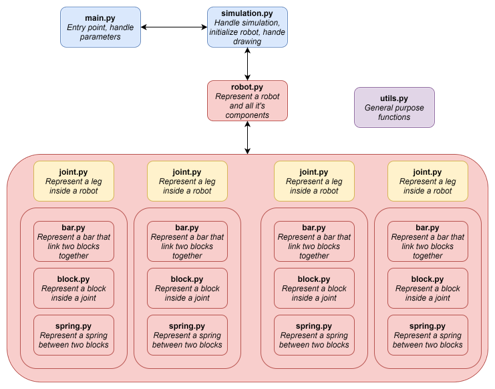
\includegraphics[width=0.7\textwidth]{images/code_structure.png}
            \caption{The simulation is structured in different modules as shown in this Figure, specifically there are modules arm, block, joint, robot, spring and simulation. The top level and entry point is the main module. Each module is responsible for its computation, drawing and constraints.}
            \label{fig:code_structure}
        \end{figure}
        
        \paragraph{arm}
            module represents the arms of a bistable joint. Those arms are connecting two blocks together with four anchors points. It is represented by two low anchors linked to the bottom block and two high anchors linked to the top block. Arm also has a length parameter. It contains functions to draw arms as output and could implement joint friction in the future. 
        \paragraph{block}
            module is the basic structure of the quadristable joint, it represents one of the three blocks, therefore it has a specific width, height, a center of mass location and anchors points to attach the arms. It also handles information about which block it represents (bottom, middle, top) and to which actuator it is connected to. This module contains functions to compute positions of anchors in addition to the drawing functions.
        \paragraph{joint}
            module represents the quadristable structure, composed of three blocks, two springs and four arms. This module contains lots of parameters, such as: joint sequence as seen in section \ref{sec:sequences}, the position of the joint relative to the main frame center of mass, the initial position of the joint, arms length ($r_1, r_2$), maximum angle ($\theta_{s1}, \theta_{s2}$) and different drawing parameters. This module first initializes the position of the different sub-modules with the input constraints such as maximum angle and arms length. It also contains the different functions that animate the legs depending of one of the 15 implemented sequences. Those sequences are based on two simple functions that take care of moving the middle block or the top block accordingly to the input.
        \paragraph{robot}
            module is responsible to build the four multistable joints, the two actuators and the main frame. It contains the joints positions relative to the robot reference frame and it coordinates the actuators motions to the multistable joints. The attitude and the position of the robot is also controlled inside this module. Each time the robot is performing a displacement, the module computes the legs touching points again and the correct orientation of the robot. This module is also responsible of drawing the main frame and the different help besides the robot drawing, such as the orientation of the robot.
        \paragraph{spring}
            module is used today only as a drawing part for the multistable joint. But it can handle future upgrades such as forces computation. 
        \paragraph{simulation}
            module is a top level part that is responsible to ensure the simulation is running correctly. It receives the different parameters from the main module and creates the robot accordingly. Once the robot is initialized, the simulation module starts to apply motion to the actuators and stores the displacement of the robot. It is also responsible to aggregate the different output points from the robot module to store them in a Pandas Dataframe which is saved for later processing. 
        \paragraph{main}
            module is a very short module that is responsible to load the configuration file that contains the parameters of the simulation and then load the simulation with this configuration.

    \section{Configuration}\label{sec:config}
        As discussed in the appendix section \ref{sec:program_structure}, the simulation is created using a configuration file. This file uses a JSON structure, which is a $key$ $value$ type of structure. There are two main categories of settings: \textit{simulation} and \textit{robot}. 
        
        The first one contains the different settings regarding the simulation process, such as \textit{actuation} field that contains the number of steps to compute, the number of cycles to simulate and the phase difference between the actuators. A phase difference of $0$° means that both actuators extend or retract at the same time. A phase difference of $180$° means that while one actuator is extending, the other is retracting itself. \textit{Draw} boolean determines if there is a video of the simulation produced. It can be useful to set it to false if we want to run the experiment fast and only create the datapoints of positions without having a video created each time. \textit{Camera\_robot\_ref} boolean allows to have a fixed camera or to have the camera that will follow the robot motion if set to true.
        
        The second group of parameters is used to initialize the robot's parameters. Each leg can be configured specifically. We have a \textit{sequence} parameter that we can set to one of the 15 sequences encoded (A-O), also the location of each leg can be customized, and also the maximum angle that a block can reach or the length of the arms.
        
    \section{Simulation process}
        The simulation process is straightforward. First it initializes the starting point of the robot and the position of each block for all the multistable legs. It also creates the actuation matrix regarding the parameters and the physical constraints of the blocks. The actuators are set to run to the maximum position they can reach with the constraints. We also dissociate the forward motion from the backward motion, which make it easier to know what motion to perform depending on the sequence.
        
        Once the initialization is done, the simulation starts with a loop that will go through all the steps of the simulation. The total number of steps is equal to $cycles \cdot steps$ and for each step it will call a function to update the position of the robot and then draw the updated position. 
        
    \section{Update robot position}
        To update the robot position, the simulation starts first to move the multistable joint individually. Each leg receives the input coming from the linked actuator and performs the correct displacement of blocks regarding the selected sequence for each leg. Once the motion from the four legs done, a function updates the attitude and the position of the robot from the displacement and position of the legs.
        First, it computes the new attitude of the robot, which is represented by a pitch (around y axis) and roll (around x axis) angles. To compute the pitch and roll angle of the robot relative to the ground, it first sorts the legs with their relative high in their own reference frame. Once done there are four possible cases. The robot can have between one and four legs that are touching the floor at the same time. Those four cases are solved in the following manner:
            \paragraph{One leg} is touching the floor. As it is not possible to get an equilibrium state on one leg, we need to look for the next leg(s) that will be touching the ground. We know that the gravity will pull the center of gravity of the robot toward the ground but it will go down with an axis of rotation that is located at the touching leg point and the rotation line will be parallel to the ground and perpendicular to the vector going from the touching leg to the center of gravity of the robot. We then look at which of the remaining leg require the smallest rotation of the robot to be touching the ground plane. The smallest angle will determine which leg(s) will then also touch the ground. There are now two, three or four touching legs and we move to the specific case respectively.
            \paragraph{Two legs in diagonal} are touching the floor. So here there are either legs one and four that are touching the ground, either legs two and three. This is a specific case where the robot is at an equilibrium state and so we can compute the roll and pitch inclination (demonstrated by experiment). 
            \paragraph{Two legs not in diagonal} are touching the floor, in this case, it needs to find a third or fourth point of contact. The process is similar to the one leg case. The center of gravity of the robot will go down and rotate around an axis. This axis is represented by a line going through the two legs that are already touching the floor. It then finds the leg that requires the smallest angle to touch the ground. We then move to the three legs case or the four legs case if both other legs are touching the floor. 
            \paragraph{Three legs} are touching the floor. To compute the pitch and roll angle, we first define the plane with three legs and compute the angle difference with the flat plane. 
            \paragraph{Four legs} are touching the floor. It is very similar to the three legs process, we just select three random legs that will create our plane to compute the roll and pitch.
            \\
            
            Once the function knows how many legs (and which) are touching the floor, it can starts to compute how legs motions translate to robot displacement. It will first compute a ratio number for each leg (d\_ratio). This displacement ratio is equal to zero if the associated leg is not touching the ground as seen in Equation \ref{eq:displacement_ratio}. This can be understood as if a leg is not touching the floor, this leg will not be able to convert its motion to the robot's displacement. The sum of the 4 displacement ratio sum to one. Then the function computes the distance of the leg to the center of gravity of the robot for each leg. To get the displacement ratio it divides the distance to the center of gravity by the sum of all the distance from legs to the center of gravity of the touching legs.

            \begin{equation}
                d\_ratio_i = 
                \begin{cases}
                  leg_i\_dist \left(\sum_{j=1;j=touch}^{n}leg_j\_dist\right)^{-1} & \text{if $leg_i$ touches the floor}\\
                  0 & \text{otherwise}\\
                \end{cases}  
                \label{eq:displacement_ratio}
            \end{equation}
            
            To get the final displacement of each leg in x-axis and y-axis a function multiplies the displacement of the leg by its displacement ratio. Then it can sum the displacement of the touching legs to get the robot's displacement.
            To compute the change robot's orientation. A function computes the angle between two vectors. The first vector represents the previous position of the leg, the second vector represents the current position of the leg in the robot's reference frame. This angle is computed with Equation \ref{eq:vector_angle}. Once all the angles are known, a function multiplies the displacement ratio to the associated angles and sum this result to get the total rotation of the robot.

            \begin{equation}
                \phi_i = sng(V_1 \wedge V_2) arctan\left(\frac{\lVert V_1 \wedge V_2 \rVert}{V_1 \cdot V_2}\right)
                \label{eq:vector_angle}
            \end{equation}
            
            With this method, if two legs are at the same distance from the robot's center of gravity and are doing an equal displacement but in opposite direction, it would produce no displacement translated to the robot. If both legs do the same displacement in the same direction, then it would give a displacement of half the displacement of both legs which gives correct results.

    \section{Displacement mapping}
        Once the simulation environment covered, the next step of the workflow is to create a controller for this multistable-based robot. To feed the controller, the workflow needs to process a table that contains different information. This is equivalent to creating a mapping table where each row will contain the sequence used by the robot, which is represented by four letters, corresponding respectively to the sequence for legs one to four. The phase difference of the actuators, which can be in phase, or in opposition of phase (0°, 180°). A boolean that represents a reverse actuation, this term is used to produce symmetric results. Finally, the table will also have the output of the simulation on each row which corresponds to the displacement in x-axis (in meters), y-axis (in meters) and the change of orientation (in rad) of the robot after one cycle. 
        To create this table a specific program is used (\textit{mapping.py}). This program runs all our realistic sequences (A-J) and tests all the possible simulations. This will produce a table off $10^4 \cdot 2 \cdot 2 = 40'000$ rows. Those rows will then be used as input or our controller.
        
    \section{Deep Q-Learning Controller}
        The implemented controller is a Deep Q-Learning controller which is based on the Reinforcement Learning (RL) principle. It is one of the most common algorithms in Reinforcement Learning. Reinforcement Learning tackle problems that involve learning how to map situations to actions to maximize a numerical reward signal\cite{sutton_barto}. First, a reinforcement learning task wants to train an agent that is interacting with an environment such as Figure \ref{fig:arena}. In this case, the \textbf{agent} is the robot, and the \textbf{environment} is a surface that contains a goal to reach. The agent is placed in an environment with different scenarios to solve. A specific position and orientation of the robot is called a \textbf{state} and the robot is able to perform \textbf{actions}, in this case the states would be for example the orientation of the robot relative to its goal and the presence of environment limits in the small signal balls around the robot. Also the actions taken from the robot would be the sequence of displacement he chooses. The agent has one purpose, it is to maximize its total reward across a \textbf{scenario} which is completed when reaching to the goal coordinates (large green dot). The policy reinforces the agent to learn to perform the best actions possible by experience. 
        
        \begin{figure}[h!]
            \centering
            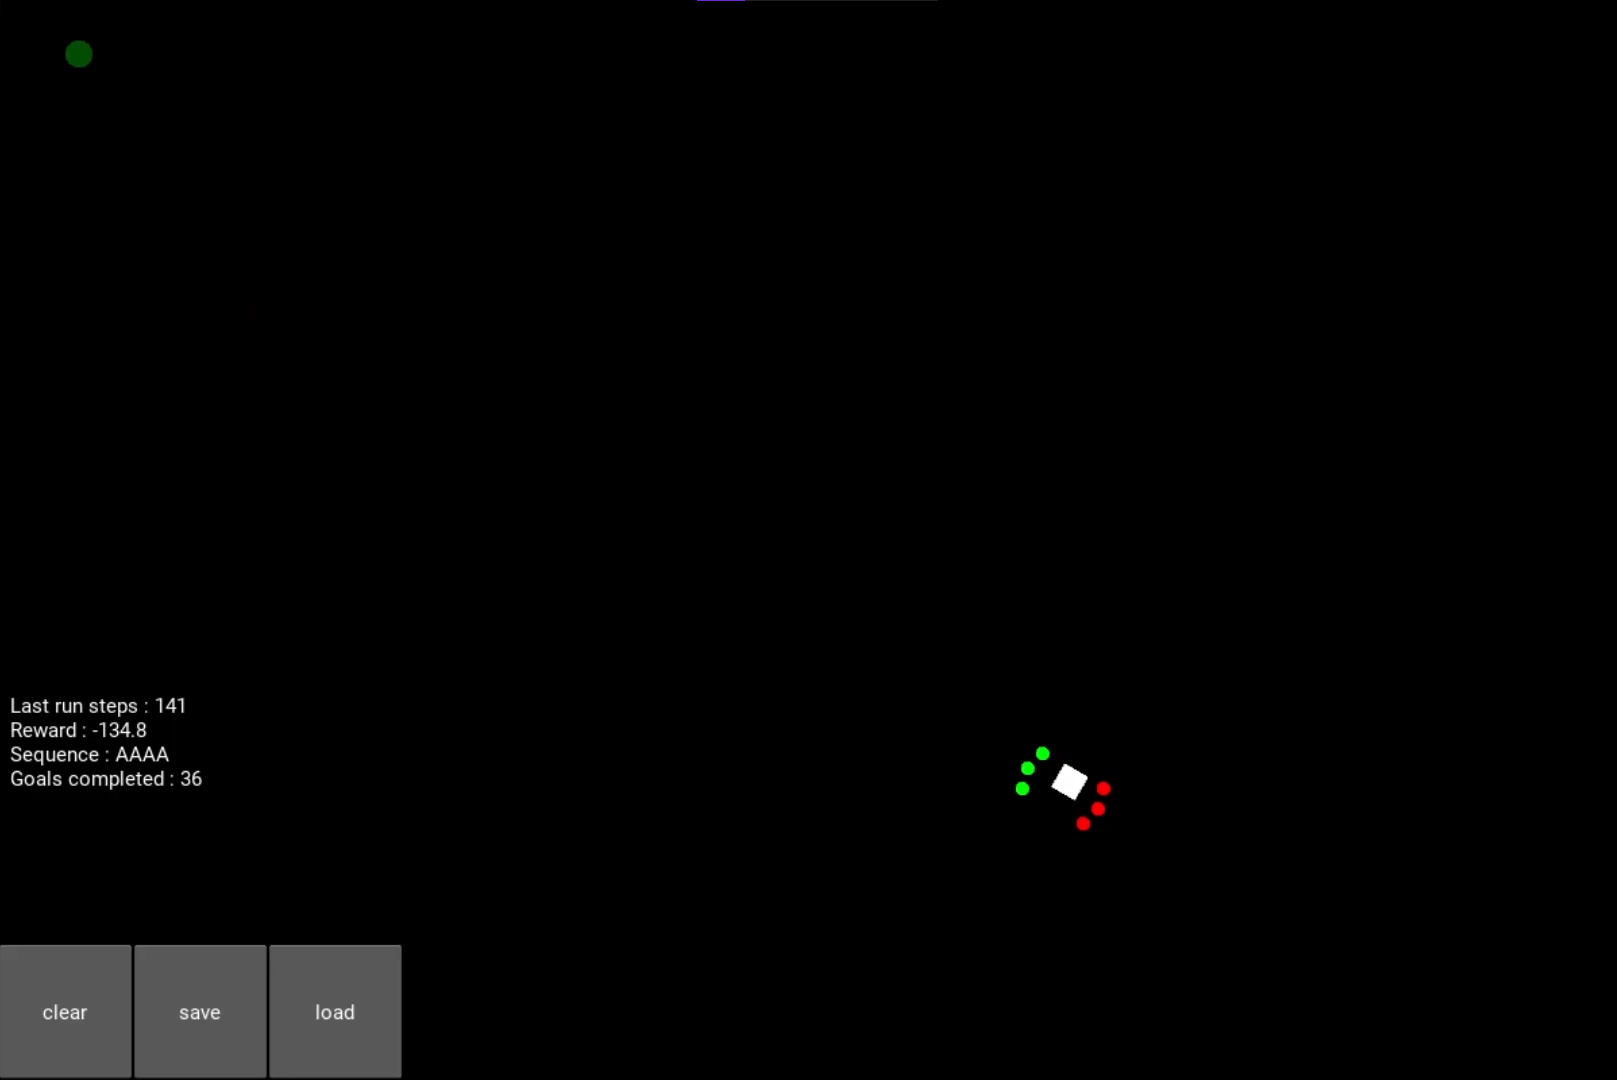
\includegraphics[width=0.66\textwidth]{images/arena.png}
            \caption{The environment in place to train a Deep Q-Learning Controller. The robot is represented by a white square and six dots, which are walls sensors. There are three green sensors in the front, three red sensors in the back. The goal of the robot is represented by a large green dot on the top left in this scenario. Once the robot reaches the goal, a new goal is set. For each action, a positive or negative reward is given depending on the consequence of the action taken by the robot.}
            \label{fig:arena}
        \end{figure}
        
        \paragraph{Q Learning}~\\
        If the expected reward is known for each action for every step, it would be possible to create a table for the agent and he would be able to understand exactly what action to perform to maximize its reward. The agent will perform the sequence of actions that will generate the maximum accumulated reward in a scenario. This accumulated reward is also called the \textbf{Q-value}. The strategy will be described as Equation \ref{eq:qlearning1}. This equation states that Q-value yielded at state $s$ and performing action $a$ is the immediate reward $r(s,a)$ added with the highest Q-value possible from the next state $s'$. The gamma term in the equation is a discount factor which controls the retention of the reward further in the future. As $Q(s',a)$ depends itself from $Q(s'',a)$, Equation \ref{eq:qlearning2} shows the Q-value depending on future states.
        Since this is a recursive equation, we can make arbitrary assumptions for all Q-values. In practical situations, this is implemented as an update equation as shown on Equation \ref{eq:qlearning3}, where alpha is the learning rate and $R$ is the reward.
        
        \begin{equation}
            Q(s,a) = r(s,a) + \gamma \max_{a}Q(s',a)
            \label{eq:qlearning1}
        \end{equation}
        \begin{equation}
            Q(s,a) \rightarrow \gamma Q(s',a) + \gamma^2 Q(s'',a) \dots \gamma^{n} Q(s'^{\dots n}, a)
            \label{eq:qlearning2}
        \end{equation}
        \begin{equation}
            Q(S_t, A_t) \leftarrow Q(S_t, A_t) + \alpha \left[ R_{t+1} + \gamma \max_{a} Q(S_{t+1}, a) - Q(S_t,A_t) \right]
            \label{eq:qlearning3}
        \end{equation}
        
        \paragraph{Deep Q Learning}~\\
        Q-Learning is a simple but already powerful algorithm to create a cheat sheet for the agent. But it can be quickly overwhelmed when the cheat sheet starts to be very long. For example in our environment there are thousands of actions per state and millions of states, this would require a table of billions of cells, which is not practical in reality. We cannot infer the Q-value of new states from already explored states. Therefore, two problems arise, first is the amount of memory required to save and update the table would increase as the number of states increases. Second, the amount of time required to explore each state to create the required table would be unrealistic. The idea of Deep Q Learning is to approximate these Q-values with Machine Learning (ML) models such as a neural network. The state is the input of the neural network and the Q-value of all possible actions is generated as the output. The different steps to create a Deep Q Learning are the following:
        \begin{enumerate}
            \item A memory stores all the past experience
            \item The maximum output of the Q-network determines the next action
            \item A loss function computes the error between the predicted Q-value and the target Q-value ($Q^*$). This consists of a regression problem.
        \end{enumerate}
        The target value can be found in Equation \ref{eq:qlearning3} with $R_{t+1} + \gamma \max_a Q(S_{t+1}, a)$. This is a value unknown as we are dealing with a reinforcement learning problem. The challenge compare to classic Deep Learning methods is that the algorithm is chasing a non stationary target, the training is not stable in a Deep Q Learning method, as it tries to learn to map for a constantly changing input and output.
        
        \paragraph{Our Controller} is using the Deep Q Learning method as the number of states and actions are high. Depending on the sequence the robot is allowed to take we have between $64$ (sequences A-B) and $202'500$ (sequences A-O) possible actions. Some filtering to remove duplicate displacement are done to reduce the number of possible actions and accelerate the learning process. The neural net used is as simple as possible with one input layer, one or two hidden layers (depending on the number of possible actions) with 64 nodes and one output layer. The loss function is a Smooth L1 Loss that use the squared term if the absolute element-wise error falls below a threshold and an L1 term otherwise. This function is less sensitive to outliers compare to Mean-Square-Error loss function and prevent gradient exploding problems.\\
        Signals that are given as input are the robot's orientation (positive and negative) relative to the goal and six signals corresponding to the signals of each dot around the robot. Those signals have a value equal to one if they are outside of the environment, zero otherwise. Lastly, we give also the reward as input of the neural net. The rewards add up as follow:
        \begin{itemize}
            \item Distance reward:
            \begin{itemize}
                \item A positive reward proportional to the distance improvement relative to the maximum displacement possible during a cycle if distance to goal decreases.
                \item A negative reward proportional to the distance deterioration relative to the maximum displacement possible during a cycle if distance to goal increases.
            \end{itemize}
            \item Orientation reward:
            \begin{itemize}
                \item $+0.2$ when current orientation is better than previous.
                \item $-0.2$ when current orientation is worse than previous.
            \end{itemize}
            \item Action persistence: $+0.02$ when the current action is the same as the previous action. As it takes time to change joint's sequence, we reward the agent when it keeps the same sequence during multiple cycles.
            \item Out of bound penalty: $-10$ when the robot is going outside the environment.
            \item Goal reached:
                \begin{itemize}
                    \item A positive reward if number of steps to reach goal is smaller than previous scenario
                    \item A negative reward if number of steps to reach goal is larger than previous scenario
                \end{itemize}
        \end{itemize}
        
            
            